\title{PmSwEng Zusammenfassung}
\author{M. Gisler}
\RequirePackage{luatex85}
\def\pgfsysdriver{pgfsys-pdftex.def}
\documentclass[a4paper]{article}

%Includes
%--------------------%
%File für alle Pakete

\usepackage{array} % Extending the array and tabular environment
\usepackage{textcomp} % Wird für Copyright-Symbol,Währungen, Musikalische-Symbole benötigt
\usepackage{graphicx}
\usepackage{tabularx}
\usepackage{mathtools} % Das mathtools package ist eine Erweiterung zum amsmath package.
\usepackage{adjustbox} %adjustbox, minipage..
\usepackage[automark]{scrpage2} % Header und Footer
\usepackage{multirow} % Create tabular cells spanning multiple rows
\usepackage{multicol} % In­ter­mix sin­gle and mul­ti­ple columns
\usepackage{rotating} % Rotation tools, including rotated fullpage floats
\usepackage{xcolor}   
%Deutsche Sprache mit Sonderzeichen und Umlauten
\usepackage[utf8]{inputenc}  % Paket für UTF-8 unterstützung
\usepackage[T1]{fontenc} %ä,ü...
\usepackage[ngerman]{babel}  %Silbentrennung und Rechtschreibung Deutsch
\usepackage{longtable}
\usepackage{wrapfig} % Randbild

% Für Code einfügen
\usepackage{listings}

%Schriftart mit LuaLatex (alle Schriften aus Word möglich)
\usepackage{fontspec}
\setmainfont{Arial}

%Schriftart mit pdflatex Compiler
%\usepackage{helvet}
%\renewcommand{\familydefault}{\sfdefault}
%\fontfamily{phv}

%Hyperlinks im Dokument
\usepackage[breaklinks,pdftex]{hyperref}
\selectfont
% Seitenränder für Formelsammlungen
\usepackage[left=1.27cm,right=1.27cm,top=0.80cm,bottom=0.80cm,includeheadfoot]{geometry}
%-----------------------------------%
%File für eigene Befehle und Makros


% Makros für Titel, Autor und Datum 
% Dank diesem Makro stehen Titel, Autor und Datum überall im Dokument zur verfügung
% Date hat zudem den Default-Wert \today
\makeatletter
\def\@Title{}
\def\@Author{}
\def\@Date{\today}
\newcommand{\Title}{\@Title}
\newcommand{\Author}{\@Author}
\newcommand{\Date}{\@Date}
\AtBeginDocument{%
	\let\@Title\@title
	\let\@Author\@author
	\let\@Date\@date
}
\makeatother

% Layout der Kopf und Fusszeile
\deftripstyle{zusammenfassung}[0pt][1.00pt]
{\Title}	% Kopfzeile innen
{}	% Kopfzeile mitte
{\Date}	% Kopfzeile aussen
{\Author}	% Fusszeile innen
{\text {Elektrotechnik@HSR}}% Fusszeile mitte
{\pagemark}	% Fusszeile aussen
\pagestyle{zusammenfassung}


%Eigene Befehle

%Befehl für Bild in Tabelle
\newcommand\tabbild[2][]{%
	\raisebox{0pt}[\dimexpr\totalheight+\dp\strutbox\relax][\dp\strutbox]{%
		\includegraphics[#1]{#2}%
	}%
}

%Befehle für linkbündig und rechtsbündig in longtable
\newcolumntype{L}[1]{>{\raggedright\arraybackslash}p{#1}} % linksbündig mit Breitenangabe
\newcolumntype{C}[1]{>{\centering\arraybackslash}p{#1}} % zentriert mit Breitenangabe
\newcolumntype{R}[1]{>{\raggedleft\arraybackslash}p{#1}} % rechtsbündig mit Breitenangabe


%%%%%%%%%%%%%%%
% Code Layout %
%https://en.wikibooks.org/wiki/LaTeX/Source_Code_Listings
%%%%%%%%%%%%%%%

\definecolor{mygreen}{rgb}{0,0.6,0}
\definecolor{mygray}{rgb}{0.5,0.5,0.5}
\definecolor{mymauve}{rgb}{0.58,0,0.82}

\lstset{ %
    firstnumber=1,
	backgroundcolor=\color{white},   % choose the background color; you must add        \usepackage{color} or \usepackage{xcolor}
	basicstyle=\footnotesize,        % the size of the fonts that are used for the code
	breakatwhitespace=false,         % sets if automatic breaks should only happen at whitespace
	breaklines=true,                 % sets automatic line breaking
	captionpos=b,                    % sets the caption-position to bottom
	commentstyle=\color{mygreen},    % comment style
	deletekeywords={...},            % if you want to delete keywords from the given language
	otherkeywords={...},             % if you want to add more keywords to the set
	escapeinside={\%*}{*)},          % if you want to add LaTeX within your code
	extendedchars=true,              % lets you use non-ASCII characters; for 8-bits encodings only, does not work with UTF-8
	frame=single,	                 % adds a frame around the code
	keepspaces=true,                 % keeps spaces in text, useful for keeping indentation of code (possibly needs columns=flexible)
	keywordstyle=\color{blue},       % keyword style
	language=C++,                    % the language of the code   
	numbers=left,                    % where to put the line-numbers; possible values are (none, left, right)
	numbersep=5pt,                   % how far the line-numbers are from the code
	numberstyle=\tiny\color{mygray}, % the style that is used for the line-numbers
	rulecolor=\color{black},         % if not set, the frame-color may be changed on line-breaks within not-black text (e.g. comments (green here))
	showspaces=false,                % show spaces everywhere adding particular underscores; it overrides 'showstringspaces'
	showstringspaces=false,          % underline spaces within strings only
	showtabs=false,                  % show tabs within strings adding particular underscores
	stepnumber=2,                    % the step between two line-numbers. If it's 1, each line will be numbered
	stringstyle=\color{mymauve},     % string literal style
	tabsize=2,	                     % sets default tabsize to 2 spaces
	%title=\lstname                   % show the filename of files included with         \lstinputlisting; also try caption instead of title
}

\lstdefinestyle{customc++}{
	belowcaptionskip=1\baselineskip,
	%frame=L,
	xleftmargin=\parindent,
	language=C++,
	basicstyle=\footnotesize\ttfamily,
	keywordstyle=\bfseries\color{blue},
	commentstyle=\itshape\color{mygreen},
	identifierstyle=\color{black},
	stringstyle=\color{gray},
}

\lstdefinestyle{git}{
	belowcaptionskip=1\baselineskip,
	%frame=L,
	xleftmargin=\parindent,
	language=C++,
	basicstyle=\footnotesize\ttfamily,
	keywordstyle=\bfseries\color{blue},
	commentstyle=\itshape\color{mygreen},
	identifierstyle=\color{black},
	stringstyle=\color{gray},
	deletekeywords={this, or, new, using, and, for, not, auto}
}

\lstdefinestyle{cppunit}{
	belowcaptionskip=1\baselineskip,
	%frame=L,
	xleftmargin=\parindent,
	language=C++,
	basicstyle=\footnotesize\ttfamily,
	keywordstyle=\bfseries\color{blue},
    keywordstyle=[2]\bf\color{black}, %not sure why \bf works, but it does
	commentstyle=\itshape\color{mygreen},
	identifierstyle=\color{black},
	stringstyle=\color{gray},
	keywords=[2]{  %Cpp Unit Keywords
		CPPUNIT_ASSERT,
       	CPPUNIT_TEST,
        CPPUNIT_TEST_EXCEPTION,
    	CPPUNIT_TEST_END,
		CPPUNIT_TEST_SUITE,
		CPPUNIT_TEST_SUITE_REGISTRATION,
        CPPUNIT_TEST_SUITE_END},
}

\lstdefinestyle{c++qt}{
	belowcaptionskip=1\baselineskip,
	%frame=L,
	xleftmargin=\parindent,
	language=C++,
	basicstyle=\footnotesize\ttfamily,
	keywordstyle=\bfseries\color{blue},
    keywordstyle=[2]\bfseries\color{red},
	commentstyle=\itshape\color{mygreen},
	identifierstyle=\color{black},
	stringstyle=\color{gray},
	keywords=[2]{           % qt-Keywords
		Qt,
		SIGNAL,
		SLOT,
		QApplication,
		QDialog,
		QGridLayout,
		QPushButton,
		QLabel,
		QVBoxLayout,
		QHBoxLayout,
		QWidget,
		QGroupBox,
		QFont,
		QLineEdit,
		QRadioButton,
		QPen,
        QRect,
        QPaintEvent,
		QBrush,
		QPixmap,
		QPainter,
        QString,
        update()},
}

\lstdefinestyle{cdoxy}{
	belowcaptionskip=1\baselineskip,
	%frame=L,
	xleftmargin=\parindent,
	language=C++,
	basicstyle=\footnotesize\ttfamily,   
	keywordstyle=\bfseries\color{blue},
   	commentstyle=\itshape\color{mygreen},
	identifierstyle=\color{black},
	stringstyle=\color{gray},
	otherkeywords={           % DoxygenKeywords
		...,
		....,
		@mainpage,
		@file,
		@author,
		@version,
		@date,
		@bug,
		@brief,
		@extended,
		@param,
		@return,
		@warning,
		@note,
		@see},
}

%choose customstyle in DOC with \lstinputlisting[style=custom]{path}
%\lstset{escapechar=@,style=customc++}
\lstset{style=customc++}


%Dokument
\begin{document}
\title{\Huge{Projektmanagement und Softwareengineering}}
\maketitle

\tableofcontents
\setcounter{tocdepth}{2} %Setzt Tiefe des Inhaltsverzeichnis
\setcounter{secnumdepth}{4} %Setzt Tiefe im Dokument selber
\thispagestyle{empty}
\newpage

\section{Software Entwicklung}
\begin{wrapfigure}[4]{r}[1pt]{3cm}
	\fbox{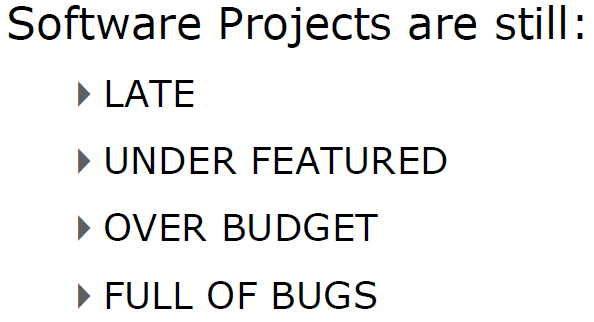
\includegraphics[width = 3.5cm]{images/softwareissues}}
\end{wrapfigure}
Die Softwareentwicklung ist schwierig,Hauptgrund: Komplexität.  
Ein Softwareprojekt kann sich aufgrund der Komplexität in einen Werwolf verwandeln. Dieser kann nur mit einer Silberkugel getötet werden.\\
Frederic Brooks hat dies analysiert: \\
\begin{itemize}
	\item \textit{"No Silver Bullet"} $\rightarrow$ Es gibt kein Wundermittel um komplexe Software zu entwickeln
	\item \textit{"{}Adding Manpower to a late Software project makes it later"}\newline
    $\rightarrow$ Neue Leute müssen sich einarbeiten und Kommunikationsaufwand steigt. 
\end{itemize}

\subsection{Schwierigkeiten/Eigenschaften}
2 Arten von Schwierigkeiten führen zu Komplexität\\ \\
\begin{tabular}{|p{0.35\linewidth}|p{0.6\linewidth}|}
	\hline
	\textbf{1. Essentielle Schwierigkeiten} & Verursacht durch Komplexität des Problems \newline Essenz: Kern der Sache
    \\ \hline
   	\quad\textbf{Eigenschaften (essential)} & Grundlegende Eigenschaften \newline \underline{Bsp.} 
    \begin{itemize}
        \item Auto muss einen Motor, Räder und Türen haben, sonst ist es kein Auto.
    \end{itemize}
    \\ \hline \hline
    
	\textbf{2. Akzidentelle Schwierigkeiten} & Selbst verursacht durch falsche Methoden, Mittel \newline Akzidenz: Art der Realisierung
    \\ \hline

	\quad \textbf{Eigenschaft (accidental)} & Zufällige Eigenschaft, die ein Objekt haben kann. \newline \underline{Bsp.} 
	\begin{itemize}
	\item Achtzylinder oder Vierzylindermotor
	\end{itemize} \\ \hline
\end{tabular}
\subsection{Bewältigung der Komplexität}	
		\begin{enumerate}
			\item Teile und herrsche \textit{"divide et impera"}
					\begin{itemize}
						\item Problem in Teilprobleme aufteilen
						\item Jedes Teilproblem für sich alleine lösen, alle zusammen ergeben die Problemlösung
						\item Möglichst eigenständige Teile (hohe Kohäsion)
						\item Möglichst geringe Abhängigkeiten (kleine Kopplung)
					\end{itemize}
			\item Abstraktion
					\begin{itemize}
						\item Definition: Weglassen von Aspekten, die für den gegenwärtigen Zweck nicht wichtig sind.
					\end{itemize}
			\item Modelle \newline
			$\Rightarrow$ visuelle Darstellung des Sachverhalts 
					\begin{itemize}
						\item Abstraktion der realen Welt, Es gibt zwei Typen von Modellen:
                        \begin{itemize}
                        \item Design-Modelle (Lösungsdarstellung)
                        \item Domain-Modelle (Problemdarstellung)
                        \end{itemize}
					\end{itemize}
		\end{enumerate}
\subsection{Magical Number Seven}
Ein Mensch kann nur gleichzeitig 7 $\pm$ 2 Informationseinheiten im Arbeitsgedächtnis präsent halten.
\subsection{Effekt des zweiten System}
Für die gewünschte Aufgabe gibt es bereits funktionsfähige Systeme, welche auch problemlos funktionieren. Das neue zweite System soll wesentlich mehr können und besser sein als das erste, ansonsten bräuchte es gar kein neues System. Dieser Ansatz führt zur \textit{"'eierlegenden Wollmilchsau"} welche alles können soll, aber sehr schwierig zu bauen ist. Dieser Effekt ist nicht nur in der Softwareentwicklung verbreitet. 
\clearpage
\subsection{Vorgehen zur Softwareentwicklung}
Wenn die folgenden Schritte gleich nacheinander durchgeführt werden, spricht man von \textit{Phasen und Phasenplänen}.
	\begin{enumerate}
		\item Analyse
			\begin{itemize}
				\item Ziel: Man weiss \textbf{\textcolor{blue}{WAS}} entwickelt werden soll.
                \subitem \rightarrow Man weiss nacher mehr als vorher
				\item Probleme, Ideen, Anforderungen aufnehmen
				\item Erstellen eines Lasten-, Pflichtenhefts und einer Anforderungsspezifikation
				\item \textit{"doing the right things"} $\rightarrow$ Die richtigen Dinge tun
			\end{itemize}
		\item Design
			\begin{itemize}
				\item Ziel: Man weiss \textbf{\textcolor{blue}{WIE}} das Produkt entwickelt werden soll
				\item Erstellen eines \textbf{\textit{Grobentwurfs}} (Festlegung der Software-Architektur, Hilfsmittel) und \newline eines \textbf{\textit{Detailentwurfs}} (UML-Diagramme). Es entsteht noch kein Code. Nur Baupläne für die Software
				\item \textit{"doing things right"} $\rightarrow$ Die Dinge richtig tun
			\end{itemize}
		\item Implementierung
			\begin{itemize}
				\item Codieren
				\item Debuggen
				\item (Testen) $\Leftarrow$ Nicht immer!
			\end{itemize}
	\end{enumerate}

\subsection{Vorgehensmodelle (Klassisch)}
\subsubsection{Begriffe}
\begin{itemize}
	\item Ein Vorgehensmodell dient dazu die Softwareentwicklung übersichtlicher zu gestalten
	\item Schwergewichtiger Prozess $\rightarrow$ Klassische Softwareentwicklung
	\item Leichtgewichtiger Prozess $\rightarrow$ Agile Softwareentwicklung
\end{itemize}

\subsubsection{Wasserfall-Modell}
\begin{minipage}{10cm}
	\begin{itemize}
		\item lineares Vorgehensmodell
		\item nicht iterativ
		\item in Realität nicht durchführbar, da keine Rückkopplung vorhanden ist
		\item Freigabe beim Abschluss jeder Phase
		\item Es gibt kein zurück, alles muss beim ersten Mal richtig gemacht werden. 
	\end{itemize}
\end{minipage}
\begin{minipage}{5cm}
	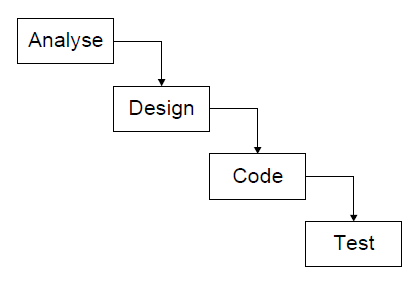
\includegraphics[width=7cm]{images/wasserfallmodell}
\end{minipage}
	
\subsubsection{Iterativer Wasserfall (Kaskade)}
	\begin{minipage}{10cm}
		\begin{itemize}
			\item Erweiterung des Wasserfalls um Korrekturschleifen
			\item In Realität durchführbar
			\item Man kann immer nur eine Phase zurück
		\end{itemize}
	\end{minipage}
	\begin{minipage}{5cm}
	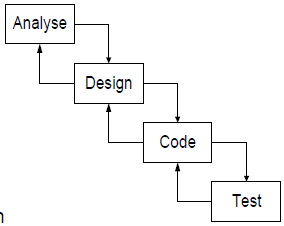
\includegraphics[width=6cm]{images/kaskade.png}	
	\end{minipage}

\subsubsection{V-Modell}
Von der deutschen Bundeswehr für ihre eigenen IT-Projekte entwickelt.\\
\begin{minipage}{8cm}
	\begin{itemize}
		\item Grundidee: Korrespondierende Tests
		\item x-Achse = Zeit
		\item y-Achse = Detaillierungsgrad
		\item Weiterentwicklung V-Modell XT,\newline
        immer projektspezifische Anpassungen nötig\newline
        (XT = Extreme Tailoring, engl. „to tailor“ = schneidern)
	\end{itemize}
\end{minipage}
\begin{minipage}{9cm}
	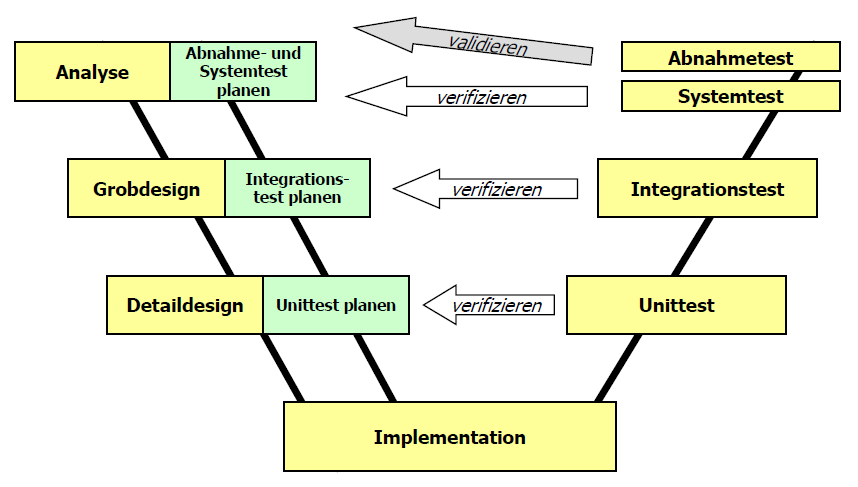
\includegraphics[width=9cm]{images/vmodell}	
\end{minipage}
\hspace{-0.5cm}
\begin{wrapfigure}[4]{r}[1pt]{7cm}
	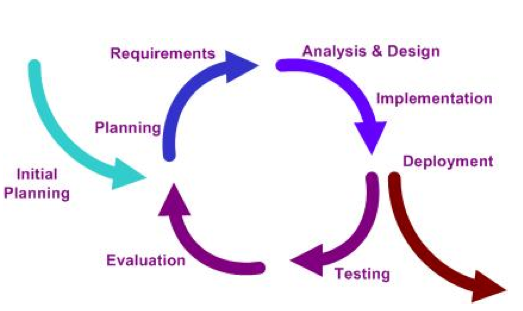
\includegraphics[width=7cm]{images/iterative_entwicklung.png}
	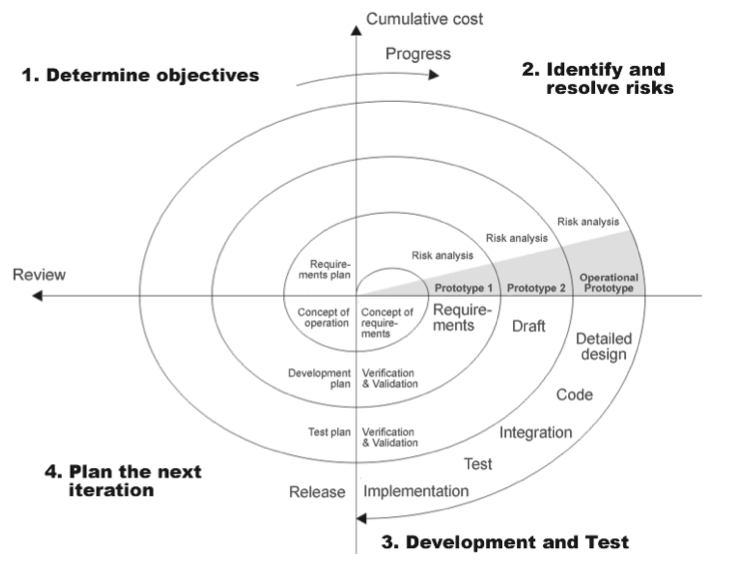
\includegraphics[width=9cm]{images/spiral_modell.png}
\end{wrapfigure}

\subsubsection{Iterative / Inkrementelle Entwicklung / Spiralmodell}
Es gibt zwei Modelle:
\begin{enumerate}
    \item Spiralmodell
    \item RUP (Rational Unified Process)
\end{enumerate}
	\textbf{Inkrementell:}
		\begin{itemize}
			\item Resultat in Schritten entwickeln
			\item Jeder Schritt ist Teil des Endresultats \newline $\Rightarrow$ wird \underline{nicht} mehr angepasst
		\end{itemize}
	\textbf{Iterativ:}
		\begin{itemize}					
			\item Erste Version entwickeln
			\item In weiteren Schritten bessere Versionen erstellen
		\end{itemize}

\subsection{Vorgehensmodelle (Agil)}
\textit{$\Rightarrow$ Ist 3 Mal erfolgreicher als das Wasserfall-Modell}
\begin{itemize}
	\item weniger formalisiert als schwerfällige, \newline
    bürokratische klassische Softwareentwicklung
	\item agil = flink, beweglich
	\item Individuen und Interaktionen gelten mehr als Prozesse und Tools
\end{itemize}
\vspace{0.5cm}
Agile Softwareentwicklung besteht aus:
\begin{enumerate}
	\item \textbf{\textit{Agile Werte:}} bilden das Fundament.\newline
	Menschen \& Interaktionen wichtiger als Prozesse \& Werkzeuge\newline
	Funktionierende Software steht über Dokumenation\newline
	Reagieren auf Veränderung anstelle von Regeln befolgen
	\item \textbf{\textit{Agile Prinzipien:}} sind Handlungsgrundsätze, die auf agilen Werten basieren.\newline
	Zufriedenstellung des Kunden durch frühe, kontinuierliche  Ausflieferung von Software\newline
	Fortschrittsmass gilt die Funktionsfähigkeit der Software
	\item \textbf{\textit{Agile Methoden:}} sind konkrete Verfahren, die sich auf agile Werte und Prinzipien stützen.
	\item \textbf{\textit{Agile Prozesse:}} sind die Zusammenfassungen angewandten Methoden.\newline
	Vorgehensmodelle wie XP, Scrum...
	\\ 
\end{enumerate}
\pagebreak
\begin{multicols}{2}
\begin{minipage}{\linewidth}
    \subsubsection{XP (Extreme Programming)}
	\begin{itemize}
		\item Bekanntester agiler Prozess
	\end{itemize}
	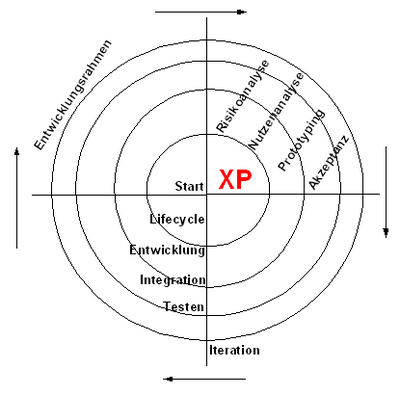
\includegraphics[width=7cm]{images/extreme_programming.png}
\end{minipage}

\begin{minipage}{\linewidth}
\subsubsection{Scrum}
$\Rightarrow$ Basiert auf sogenannten User Stories (Use Cases)\\
	\begin{itemize}
		\item Gedränge
		\item \textit{\textbf{Basis:}} Sprints von 15-30 Tagen, in welchen vom Team eine neue (bessere) Softwareversion erstellt wird. 
	\end{itemize}
	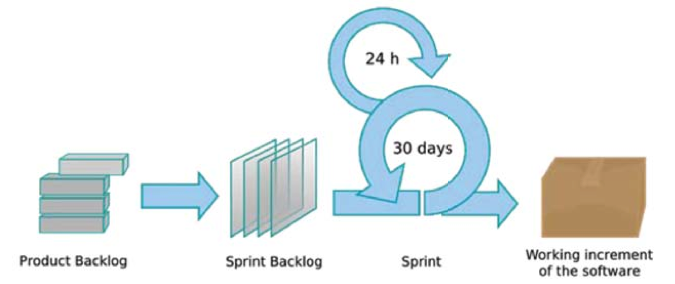
\includegraphics[width=10cm]{images/scrum.png}
\end{minipage}
\\
\end{multicols}

\subsection{Objektorientierte Softwareentwicklung (OOAD)}
\begin{minipage}[b]{13cm}
	\begin{itemize}
		\item Modelle auf allen Stufen:\textcolor{blue}{\textbf{ OO-Analyse $\rightarrow$ OO-Design $\rightarrow$ OO-Implementation}}
		\item \textit{Objekte} sind Abstraktionen von realen Dingen (Modellen)
		\item Klassen entstehen durch Gruppieren und Zusammenfassen von Objekten mit gleicher Datenstruktur
		\item Gleiche Notation bei OOA, OOD, OOI
		\item Darstellung mit UML
		\item OOAD kann in jedem Vorgehensmodell verwendet werden
	\end{itemize}
	\vspace{1pt}
\end{minipage}
\newline
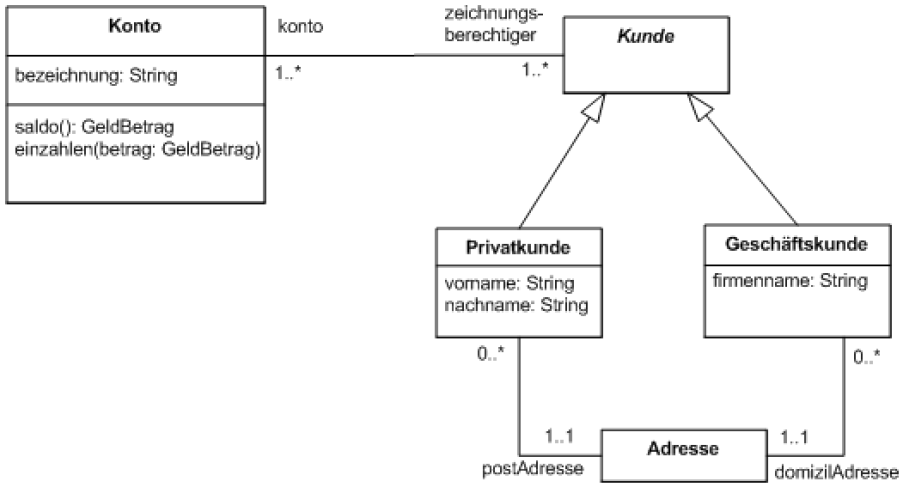
\includegraphics[width=12cm]{images/uml.png}

\begin{multicols}{2}
\subsection{Kriterien für die Wahl des Modells}
\begin{itemize}
	\item Projektgrösse
	\item Projektkomplexität
	\item Verfügbarkeit der Ressourcen
	\item Zeitpunkt von Änderungen (diskret, laufend)
	\item Qualität der Anforderungsdefinitionen
	\item Stabilität bzw. Volatilität der Anforderungen
\end{itemize}

\subsection{The Big Bang Problem bei Wasserfallmodellen}
\begin{enumerate}
	\item zuerst lange Analyse-Phase mit dem Kunden
	\item dann lange Phase für Design, Codierung und Test \newline $\rightarrow$ Kein Kundenkontakt
	\item Einführung des Systems beim Kunden $\Leftarrow$ \textcolor{blue}{\textbf{Big Bang}} 
	\item \textbf{Folge:} Hektisches Nachbessern
\end{enumerate}
$\Rightarrow$ \textit{Häufig wird dadurch das Vertrauen des Kunden zerstört.}
\end{multicols}
\clearpage
\section{Testing}
\subsection{Allgemeine Begriffe}
\begin{itemize}
	\item Definition: Programm mit der Absicht ausführen, Fehler zu finden. 
	\item Durch das Testen kann die Korrektheit eines Programms nicht bewiesen werden!
	\item Mit Testen kann nur die Anwesenheit von Bugs bewiesen werden, aber nicht die Abwesenheit. 
	\item Erster Bug: 1947 wurde eine Motte im Relais eines Mark II Aiken Rechners entdeckt.
\end{itemize}

\textbf{Wahrscheinlichkeit von Fehlern}\\
\begin{minipage}{12cm}
Je mehr Fehler gefunden werden, desto höher ist die Wahrscheinlichkeit weiterer Fehler.
\end{minipage}
\begin{minipage}{6cm}
	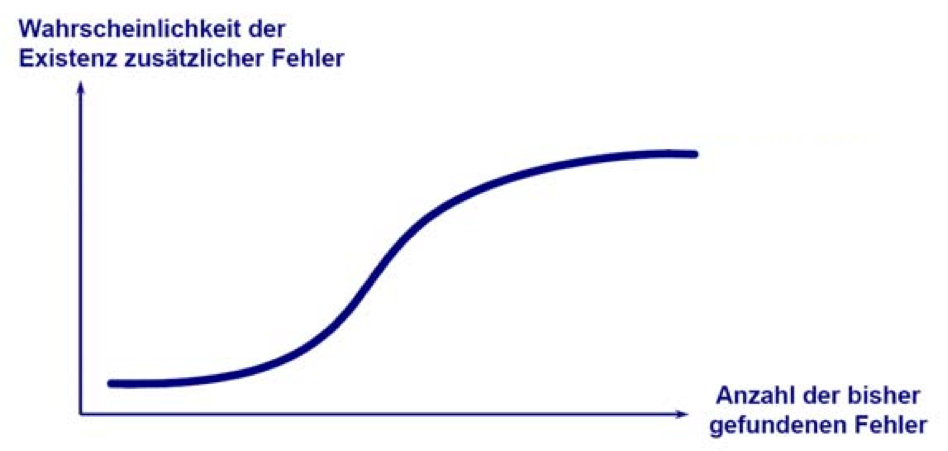
\includegraphics[width=6cm]{images/fehler_wkeit.png}	
\end{minipage}

\begin{multicols}{2}
	\subsubsection{Verifikation \& Validierung}
	\textbf{Validierung:}\\
	\textit{"{}Are we building the right product?"}\\
	Überprüft das Produkt ob es die Anforderungen des Auftraggebers erfüllt.\\
	\textbf{Verifikation:}\\
	\textit{"{}Are we building the product right?"}\\
	Überprüft ob die erstellte Software funktioniert.\\
	
	\subsubsection{Testen \& Debuggen}
	\textbf{Ziel des Testing:} \\
	Aufzeigen, dass Fehler existieren.\\
	\textit{"{}Jeder gefundene Bug ist ein Gold Nugget"}\\
	\textbf{Ziel des Debugging:} \\
	Durch Testing gefundene Fehler lokalisieren und beheben.
	
\end{multicols}

\begin{multicols}{2}	
\subsubsection{Anforderungen an Softwaretests}
	\begin{minipage}{12cm}
	\begin{itemize}
			\item Geplant $\rightarrow$ Testplan erstellen
			\item Systematisch $\rightarrow$ Testspezifikationen erstellen
			\item Festgehalten $\rightarrow$ Testprotokoll erstellen
			\item Reproduzierbarkeit:
			\begin{itemize}
				\item Wissen, was getestet wurde
				\item Unabhängig von testender Person
			\end{itemize}
			\item Automatisierung, wenn möglich
			\item Testspezifikationen laufend erweitern,\\
			Regressionstests
		\end{itemize}
	\end{minipage}
		\begin{minipage}{10cm}
			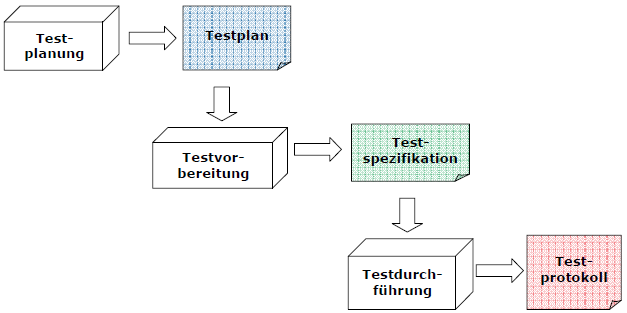
\includegraphics[width=10cm]{images/sofwaretest.png}
		\end{minipage}
\end{multicols}

\begin{multicols}{2}
	\subsubsection{Massnahmen zur Softwareprüfung}
	\begin{itemize}
		\item Dynamische Prüfung
		\begin{itemize}
			\item Testing
			\item Dynamische Analyse
		\end{itemize}
		\item Statische Prüfung
		\begin{itemize}
			\item Metrikanalyse
			\item Code Reviews
		\end{itemize}
	\end{itemize}
	
	\subsubsection{Arten von Tests}
	\begin{itemize}
		\item Funktionale Tests
		\item Nicht-Funktionale Tests
		\begin{itemize}
			\item Leistungstests
			\item Usability Tests
			\item ...
		\end{itemize}
	\end{itemize}
\end{multicols}

\pagebreak
\subsection{Testmethoden}
\subsubsection{Blackbox Tests}
	Tests ohne Kenntnis der inneren Struktur;\\

\textbf{Äquivalenzklassen:} \\
\begin{minipage}{15cm}
Wertebereich, für welche das Programm voraussichtlich das gleiche Verhalten zeigt. \\
Methodik: 1 Testcase pro Äquivalenzklasse \\
Beispiel: Quadratische Gleichung; Determinante $<0$ ; $=0$ ; $>0$ \\
\end{minipage}
\begin{minipage}{4cm}
	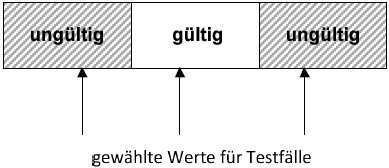
\includegraphics[width=4cm]{images/aequivalenzklasse.png}
\end{minipage}

\textbf{Grenzwertanalyse:} \\
\begin{minipage}{12cm}
Fehler liegen oft an Grenzen zulässiger Eingabewertbereiche. \\
Methodik: Testfälle auf Grenzen und knapp daneben \\
\end{minipage}
\begin{minipage}{4cm}
	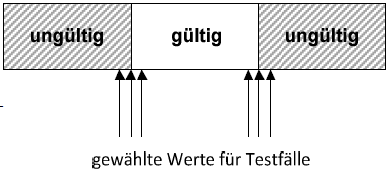
\includegraphics[width=4cm]{images/grenzwertanalyse.png}
\end{minipage}

\textbf{Zustandsbasiertes Testing:} \\
Beispiel Stack: \\
Zustände: Stack leer, Stack halb-voll, Stack voll \\
Testfälle: Element hinzufügen, Element entfernen

\subsubsection{Whitebox Tests}
\begin{minipage}{13cm}
Tests mit Kenntnis der inneren Struktur;\\
Whitebox-Test werden mittels Kontrollfluss-Graphen durchgeführt. \\
Jedes Statement entspricht Knoten.\\
Zweige, stellen Schleifen und Verzweigungen dar, verbinden Knoten. \\
Der Test wird so ausgelegt, dass die Überdeckung (Coverage) möglichst gut ist. (Test der Überdeckung mit Dynamic Analyzer)
\end{minipage}
\begin{minipage}{5.5cm}
	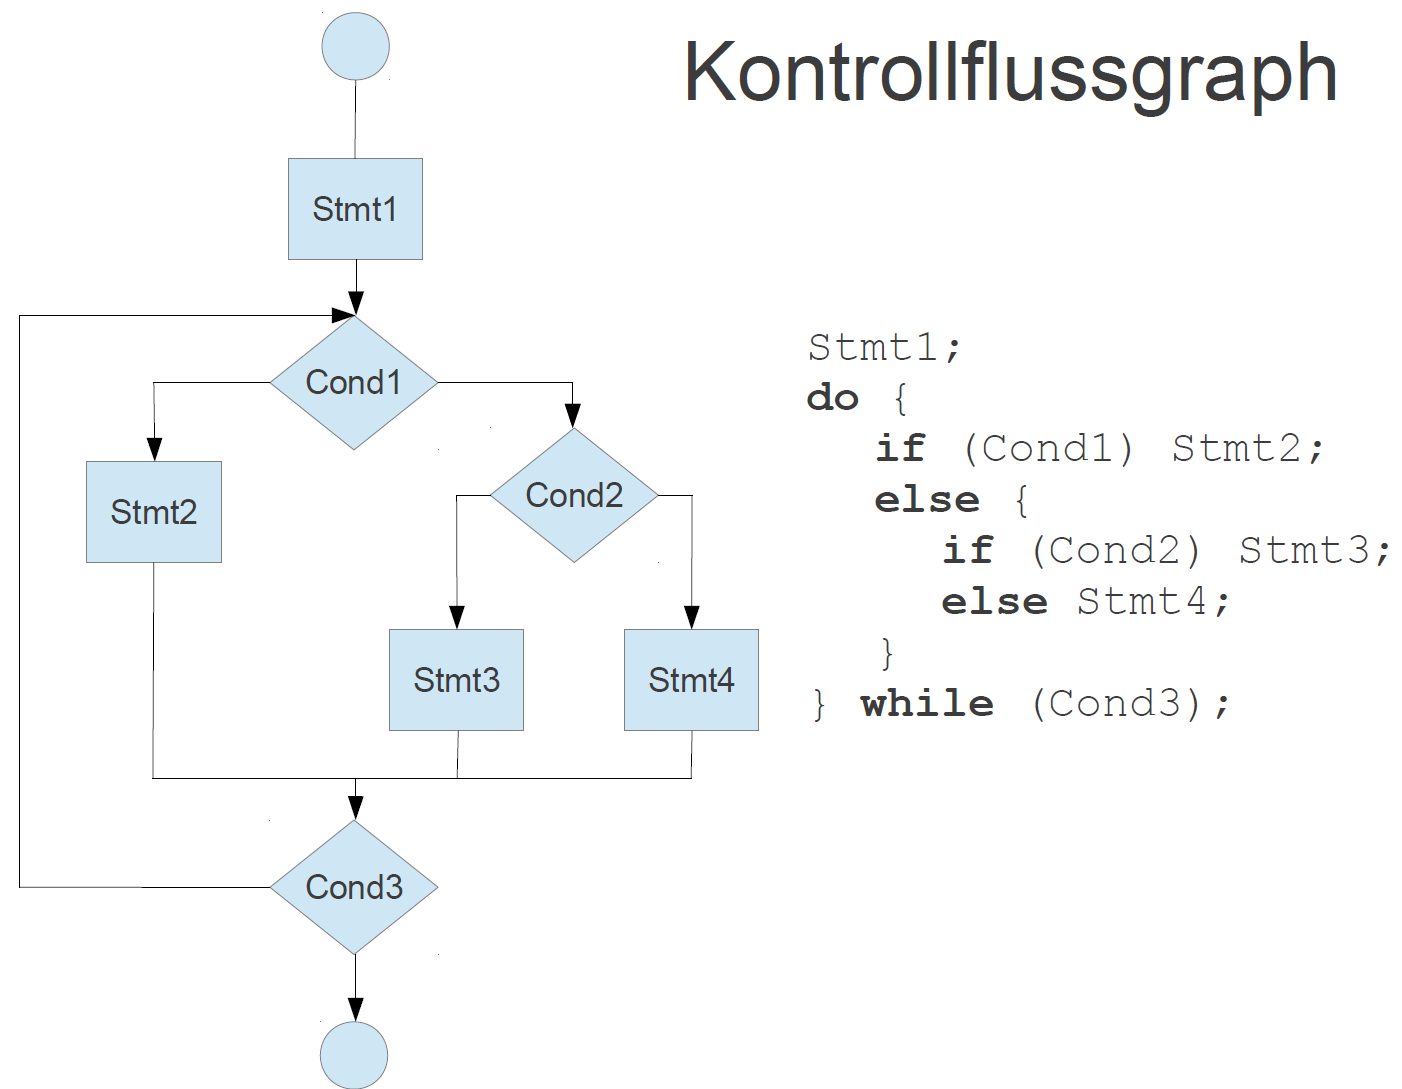
\includegraphics[width=5.5cm]{images/kontrollflussgraphen.png}
\end{minipage}

\begin{itemize}
	\item Anweisungsüberdeckung (statement coverage)
			\begin{itemize}
				\item Prozentualer Anteil der Anweisungen welche im Test ausgeführt werden
				\item 100\% Anweisungsüberdeckung ist Minimum
			\end{itemize}
	\item Zweigüberdeckung (branch coverage)
			\begin{itemize}
				\item Prozentualer Anteil der Zweige welche durchlaufen werden
				\item 100\% Zweigüberdeckung $\Rightarrow$ 100\% Anweisungsüberdeckung
			\end{itemize}
	\item Bedingungsüberdeckung
			\begin{itemize}
				\item Verschiedene Kombinationen testen bei zusammengesetzten Bedingungen
				\item mind. 1x true/false durchlaufen
			\end{itemize}
	\item Pfadüberdeckung (path coverage)
			\begin{itemize}
				\item Prozentualer Anteil der Pfade welche im Test durchlaufen werden
				\item Ein Pfad ist möglicher Weg durch Kontrollgraphen
			\end{itemize}
	\item Funktionsüberdeckung
			\begin{itemize}
				\item \textit{"{}Tut es das, was der Kunde spezifiziert hat?"}
				\item 1 Szenario pro Use Case 
				\item Blackbox Tests
			\end{itemize}
\end{itemize}

\subsection{Testwerkzeuge}
\begin{tabular}{ll}
	Blackbox: & FIT \\
	Whitebox: & xUnit
\end{tabular}


\subsection{Automatisiertes Testing}
\textbf{Vorteile:}
\begin{itemize}
	\item Wiederholbarkeit (Regressionstests möglich)
	\item Eindeutige Spezifikationen (Testcode ist Programmcode)
\end{itemize}	
\textbf{Nachteile:}
\begin{itemize}
	\item Mehr Code zu schreiben und zu pflegen
	\item Testcode ist Programmcode: Wird überhaupt das Richtige getestet?
\end{itemize}

\subsection{Unit-Test}
\subsubsection{Konzept}
\begin{minipage}{10.5cm}
	\begin{itemize}
		\item Test einer Komponente (Unit)
		\item Testen der Schnittstelle der Unit
		\item automatisch wiederholbar
		\item mittels Unit-Test-Frameworks \\
		Frameworks: Programmgerüst in welches das Anwendungsprogramm eingebettet wird. Die Funktionen der Unit werden aus dem Framework heraus aufgerufen, sogennantes Hollywood-Prinzip:\\
		\textit{"{}Don't call us, we'll call you"}
	\end{itemize}
\end{minipage}
\begin{minipage}{9cm}
	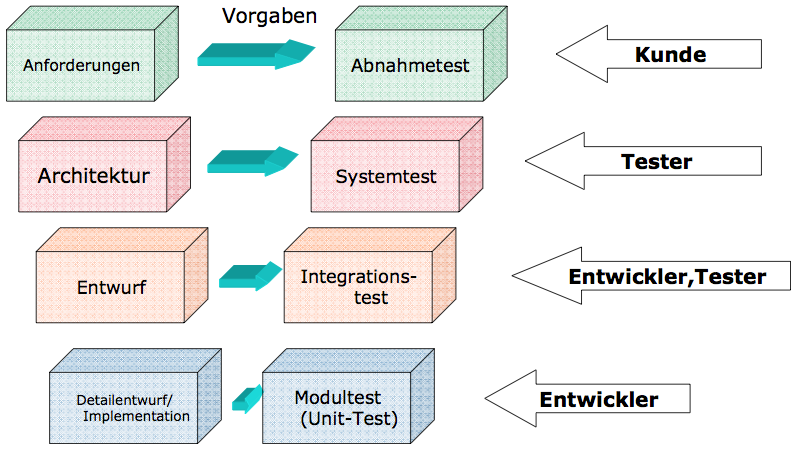
\includegraphics[width=9cm]{images/wer_testet.png}
\end{minipage}

\subsubsection{Arbeitsweise}
\begin{itemize}
	\item Spezielle, möglichst einfache Testfunktion mit Zusicherungen
	\item Test-Run endet mit OK oder FAILED
\end{itemize}

\subsubsection{Vorteile}
\begin{itemize}
	\item Tests sind aufgeteilt, pro Klasse eine Testklasse
	\item Innerhalb der Datei in Testfunktion und Testsuite
	\item Testprotokollausgabe möglich 
\end{itemize}

\subsubsection{Unit-Test mittels CPPUNIT}
\begin{minipage}{15cm}
	\begin{itemize}
		\item Assert-Anweisung, vergleicht Soll mit Ist
		\item Test-Runner Programm das die Test-Funktionen nacheinander ausführt
		\item Testklasse, selbstgeschriebene Klasse die vom Testcase erbt
		\item Testfunktion, enthält Assert-Anweisungen
		\item Testsuite, fasst Testfunktionen zusammen
		\item Testfixture Bereitstellung und Abbau einer Testumgebung
		\item Beispiel im Anhang
	\end{itemize}
\end{minipage}

\pagebreak
\section{Dokumentation \& Doxygen}
\subsection{Dokumentation}
\subsubsection{Zweck der Dokumentation}
\begin{itemize}
	\item Wissenssicherung / Wissenstransfer
	\item Kommunikation
	\item Sichtbarkeit des Projektfortschritts
\end{itemize}
\subsubsection{Dokumentation von Software}
\begin{minipage}{\linewidth}
\begin{itemize}
	\item Benutzung von bestehenden Programmteilen \newline $\rightarrow$ Schnittstellenbeschreibung (API, Application Program Interface)
	\item Zielgruppe ist Programmierer
	\item Dokumente werden oftmals nicht nachgeführt, wenn Änderungen am Sourcecode gemacht werden $\rightarrow$ Inkonsistenz \newline $\rightarrow$ Programmdokument ist fehlerhaft und verliert dadurch an Wert.
	\item Im Sourcecode werden mittels speziell gekennzeichneten Kommentaren Beschreibungen erstellt.
	\item Mittels Dokumentationswerkzeugen kann Kommentar Source-Code extrahiert werden und daraus eine Beschreibung erstellen.  
\end{itemize}
\end{minipage}
\subsection{Doxygen}
Doxygen ist ein solches Dokumentationswerkzeugen wie oben erwähnt. Es erstellt API-Beschreibungen.\\
Es ist weit verbreitet und Open-Source. (Beispiel im Anhang)
\begin{itemize}
	\item unterstütze Sprachen: C,C++,Java, C\#,...
	\item Ausgabeformate: HTML, LaTeX, RTF, XML,...
	\item auch UML-Diagramme möglich
	\item Ist grundsätzlich ein Command Line Tool
	\item Hauptbefehl (command-line): \texttt{\$ \textcolor{blue}{doxygen}}
	\item existiert aber auch ein GUI und ein Eclipse-Plugin (Eclox, in Eclipse das Symbol @)
	\item benötigt Konfigurationsdatei \"{}Doxyfile\"{} \newline
	 $\rightarrow$ \"{}Doxygen\"{} ist sehr umfangreich: rund 70.. 100 Optionen. \newline $\rightarrow$ Wichtigster Parameter: \texttt{PROJECT\_NAME} 
	\item im File Doxyfile sind alle Einstellungen gespeicher was alles in die Dokumentation muss
\end{itemize}
%\begin{multicols}{2}
    \renewcommand{\arraystretch}{1.3}
    \begin{minipage}{0.5\linewidth}
        \subsubsection{Doxygen Commands}
        \begin{tabular}{|l|l|}
        	\hline	/** DoxyCmt */  &  Doxygen Comment\\ 
        	\hline	@file	      	& File Name. Next Line Description of the File.\\
        	\hline	@author 	    & Author\\
        	\hline	@version	    & Version \\
        	\hline   @date		    & Datum   \\ 
        	\hline   @bug    		& A known Bug \\
        	\hline   @brief	    	& One Line description  \\
        	\hline   @extended	    & Description over several Lines  \\
        	\hline   @param	       	& Description of your Parameter  \\
        	\hline   @return	    & Description of your Returnvalue     \\ 
        	\hline   @warning	    & Warnings \\ 
        	\hline   @note		    & Note\\ 
        	\hline        
        \end{tabular}
    \end{minipage}
    \hspace{1cm}
    \begin{minipage}{0.5\linewidth}
        \subsubsection{Aufruf-Beispiele}
        \begin{itemize}
            \item \texttt{doxygen} // gibt Hilfe-Text aus
            \item \texttt{doxygen -g}           // erzeugt Konfig.-Datei \"{}Doxyfile\"{}
            \item \texttt{doxygen Doxyfile}     // erzeugt Dokumentation
        \end{itemize}
    \end{minipage}
%\end{multicols}
\clearpage
\subsubsection{Doxygen Architektur}
\vspace{3cm}
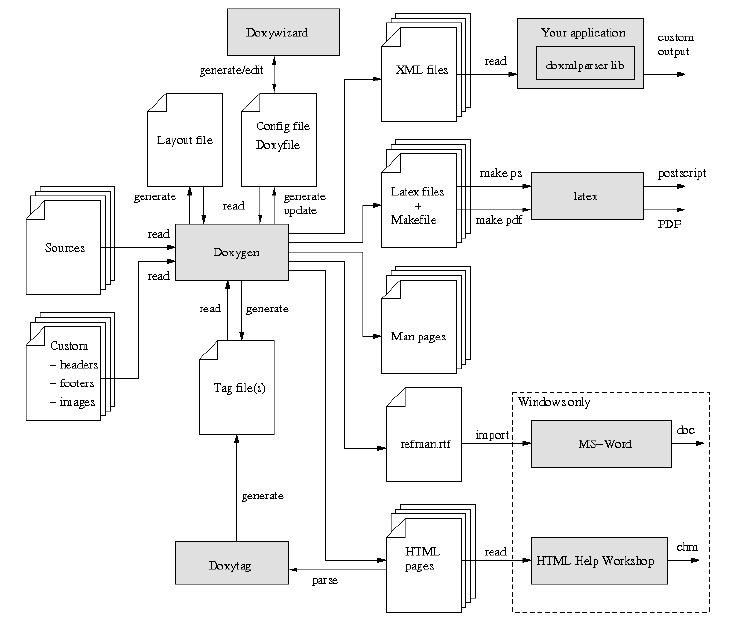
\includegraphics[width = 1.2\linewidth, angle = 90]{images/doxygen}
\clearpage

\pagebreak
\section{Projektmanagement}
\subsection{Grundlagen}

\subsubsection{Definition eines Projektes}
Ein Projekt ist ein zeitlich beschränktes Vorhaben zur Erzeugung eines einmaligen Produkt oder Dienst. 

\subsubsection{Definition des Projektmanagement}
Das Projektmanagement bezeichnet die Gesamtheit von Führungsaufgaben, -organisation, -techniken und -mitteln für die Initiierung, Definition, Planung, Steuerung und den Abschluss von Projekten. 

\begin{multicols}{2}
	\subsubsection{Merkmale eines Projektes}
	\begin{itemize}
		\item einmaliges Vorhaben
		\item klare Ziele
		\item hat Risiken
		\item zeitlich begrenzt
		\item Kostenrahmen
		\item hat innovativen Charakter
		\item es arbeiten mehrere Personen daran
		\item hat Projektleiter \& Projektteam 
	\end{itemize} 
	
	\subsubsection{Kategorien von Projekten}
	\begin{itemize}
		\item Forschungs- und Entwicklungsprojekte
		\begin{itemize}
			\item  Entwicklung neuer Produkte
			\item  Erstellung von Software
		\end{itemize}			 
		\item Investitionsprojekte
		\begin{itemize}
			\item Bau eines Flughafen			
		\end{itemize}
		\item Organisationsprojekte
		\begin{itemize}
			\item Einführung Software
			\item Vorbereitung Veranstaltung
		\end{itemize}
	\end{itemize}
\end{multicols}

\subsubsection{Die 3 Eckpfeiler eines Projektes}
\begin{minipage}{10cm}
	Diese drei Grössen sind voneinander abhängig und sind auch bekannt als \textit{"Fast, Good, Cheap"}
	\begin{itemize}
		\item Ergebnis \textit{"Scope"}
		\item Zeit \textit{"Time"}
		\item Aufwand \textit{"Cost"}
	\end{itemize}
\end{minipage}
\begin{minipage}{3cm}
	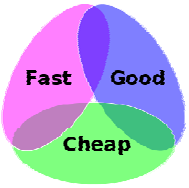
\includegraphics[width=3cm]{images/eckpfeiler.png}
\end{minipage}
\begin{minipage}{3cm}
	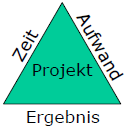
\includegraphics[width=3cm]{images/dreieck.png}
\end{minipage}

\subsubsection{Das Projektdreieck (Magisches Dreieck)}
\begin{minipage}{15cm}
	Diese drei Grössen werden als Dreieck dargestellt. Die Aufgabe des Projektmanagement ist es, ein sinnvolles Verhältnis dieser 3 herzustellen und während der Projektdauer zu gewährleisten. 
\end{minipage}

\subsubsection{Projektbeteiligten (Stakeholder)}
\begin{itemize}
	\item Auftraggeber $\rightarrow$ bezahlt \& befiehlt
	\item Projektleiter (PL) $\rightarrow$ Manager, weniger Fachexperte
	\item Projektmitarbeiter (Projektteam) $\rightarrow$ Fachexperten, hohe Methoden und Sozialkompetenz
\end{itemize}

\subsubsection{Projektorganisationsformen}
\begin{multicols}{3}
	\begin{itemize}
		\item \textbf{Reine Projektorganisation}
		\begin{itemize}
			\item Projektleiter \& Projektteam arbeiten Vollzeit am Projekt
			\item Mitarbeiter sind voll\-kommen Projektleiter \newline unterstellt
			\item sehr selten
		\end{itemize}
		\item \textbf{Matrix-Projektorganisation}
		\begin{itemize}
			\item Mitarbeiter arbeiten Teilzeit am Projekt
			\item Verantwortung ist aufgeteilt zwischen\newline Projektleiter/Linieninstanzen
			\item Häufigste Form
		\end{itemize}
		\item \textbf{Stabs-Projektorganisation}
		\begin{itemize}
			\item Hierarchie ist unverändert
			\item Projektkoordinator hat \newline keine Weisungsbefugnisse
			\item stimmt Zusammenarbeit mit Mitarbeiter ab
		\end{itemize}
	\end{itemize}
\end{multicols}

\subsection{Projektablauf}
Jedes Projekt hat ein Anfang und ein Ende (Lebenszyklus). Der vorzeitige Abbruch ist ein Unfall, sogenanntes \newline ungeplantes Ende. Jedes Projekt besteht aus 4 Phasen. Die 4 Phasen überlappen sich und laufen parallel ab. \newline Während der Durchführung ist auch die Planung anzupassen. \\
\\
\begin{minipage}{6cm}
	\textbf{Projektphasen:}
	\begin{enumerate}
		\item Projektdefinition
		\item Projektplanung
		\item Projektdurchführung
		\item Projektabschluss
	\end{enumerate}
\end{minipage}
\begin{minipage}{7cm}
	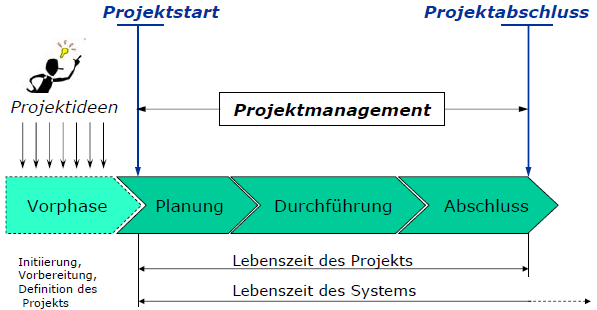
\includegraphics[width=8cm]{images/projektablauf.png}
\end{minipage}

\subsection{Projektphasen}
Verschiedene Teilprozesse laufen parallel ab. 
\subsubsection{Projektdefinition (Vorphase, Initiierung)}
\begin{itemize}
	\item Vorbereiten des Projektes
	\item Vor dem eigentlichen Projekt
	\item Ziele festlegen (Das Wichtigste eines Projektes)
	\item Termine, Kosten und Projektorganisation festlegen
	\item Wird in Projektauftrag niedergeschrieben
\end{itemize}
	\begin{minipage}{11cm}
		\textbf{Projektauftrag} \\
		Der Projektauftrag ist ein schriftliches Dokument wo Ziele und Rahmenbedingungen festgehalten sind. Das Dokument wird vom Auftraggeber unterzeichnet, damit ist Existenz des Projektes formell bestätigt. \newline Die Ziele des Projektes sollten gemäss SMART formuliert sein. 
	\end{minipage}
	\begin{minipage}{6cm}
		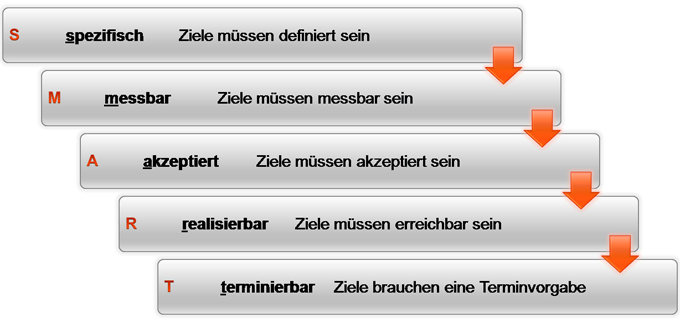
\includegraphics[width=6cm]{images/smart.png}
	\end{minipage}
	
\subsubsection{Projektplanung}
Als Voraussetzung zur Projektplanung gilt der erstelle Projektauftrag. Anschliessend findet das \textit{"Kick-Off-Meeting"} statt. Es ist das erstmalige Treffen des ganzen Projektteams, nachher ist das Team arbeitsfähig. Das \textit{"Kick-Off-Meeting"} gilt als offizieller Projektstart.\\
Die Projektplanung ist das Wichtigste. Die Pläne werden periodisch überarbeitet weil niemals alles nach Plan läuft. 
\vspace{0.2cm}
\\
\begin{minipage}{11cm}
	\textbf{1. Projektstrukturplan (PSP)}
	\begin{itemize}
		\item Projekt in Teilprojekte zerlegen
		\item Kleinstmögliche Aufgaben sind Arbeitspakete
		\item Arbeitspakete sind phasenorientiert (nach Zeitabschnitten) oder objektorientiert (nach Komponenten) oder funktionsorientiert (nach Ähnlichkeit der Aufgaben) aufgeteilt
		\item Pro Arbeitspaket wird eine Arbeitsbeschreibung erstellt
	\end{itemize} 	
\end{minipage}
\begin{minipage}{7cm}
	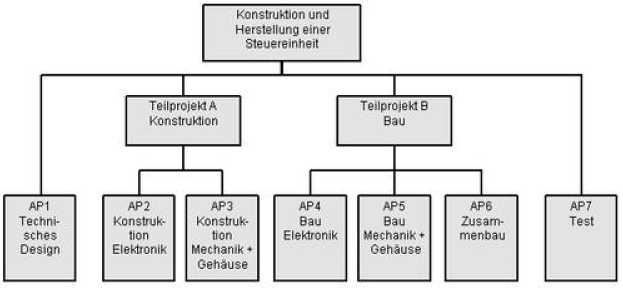
\includegraphics[width=7cm]{images/projektstrukturplan.png}
\end{minipage}
\clearpage
\pagebreak
\textbf{2. Projektablaufplan (PAP)} \\
Stellt die logische Abhängigkeiten der Arbeitspakete dar. Dazu wird eine Vorgangsliste erstellt, welche die Abhängigkeiten zwischen den Arbeitspakete aufzeigt. 
\renewcommand{\arraystretch}{1.2}
\begin{table}[h!]
	\begin{tabular}{|l|l|l|}
		\hline \textbf{Abhängigkeit} & \textbf{Funktion} & \textbf{Bild} \\
		\hline Normalfolge & Nachfolger kann erst beginnen, wenn Vorgänger beendet ist & \tabbild[width=4cm]{images/normalfolge.png}\\
		\hline Anfangsfolge & Nachfolger kann erst beginnen, wenn Vorgänger begonnen hat &
		\tabbild[width=4cm]{images/anfangsfolge} \\
		\hline Endfolge & Nachfolger kann erst enden, wenn Vorgänger beendet ist &
		\tabbild[width=4cm]{images/endfolge.png} \\
		\hline Sprungfolge & Nachfolger kann erst enden wenn Vorgänger begonnen hat &
		\tabbild[width=4cm]{images/sprungfolge.png}\\
		\hline
	\end{tabular}
\end{table}

\textbf{3. Projektterminplan}
\begin{itemize}
	\item Zuordnung von Terminen zu Arbeitspaketen
	\item Festlegen der Meilensteine
    \begin{itemize}
    	\item Meilensteine sind Etappenziele welche zur Projektkontrolle dienen
    	\item Meilensteine sind so formuliert, dass \textit{"'Erfüllt"} oder
    	\item Meilensteine stehen am Ende jeder Projektphase
    	\textit{" Nicht Erfüllt"} gilt
    \end{itemize}
	\item Projektterminplan wird aufgrund des PSP und PAP erstellt
\end{itemize}
\begin{table}[h!]
	\begin{tabular}{l l l}
		 \textbf{Balkendiagramm} & \textbf{Netzplan} & \textbf{Microsoft Project} \\
		 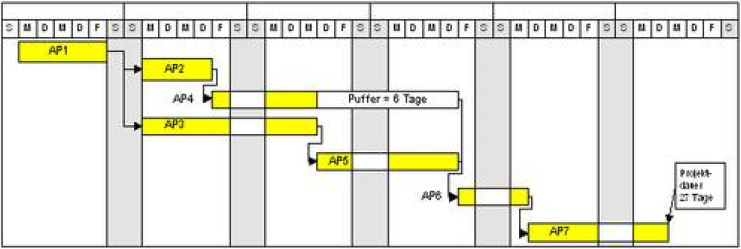
\includegraphics[width=6cm]{images/balkendiagramm} & 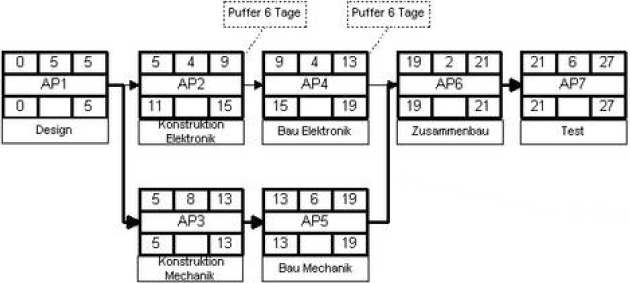
\includegraphics[width=6cm]{images/netzplan}	& 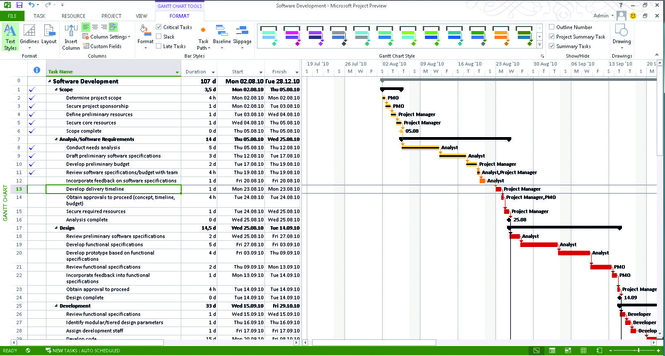
\includegraphics[width=6cm]{images/msproject}	 
	\end{tabular}
\end{table}
\vspace{0.2cm}
\textbf{4. Ressourcen- und Kapazitätsplan}\\
Die benötigten Ressourcen ermitteln und mit den Kapazitäten abstimmen. 
\\
\\
\textbf{5. Kosten- und Budgetplan}\\
Die Kosten für für die Ressourcen schätzen und Budget erstellen. 

\subsubsection{Projektdurchführung}
Die eigentliche Arbeit beginnt. Der Projektleiter hat die Aufgabe des Projekt-Controlling (to control $\rightarrow$ steuern).\\
Projekt-Controlling = Projektkontrolle + Projektsteuerung 
\renewcommand{\arraystretch}{1.2}
\begin{table}[h!]
	\begin{tabular}{|l|l|}
		\hline \textbf{Projektkontrolle} 	& Rechtzeitiges Feststellen von Abweichungen gegenüber dem geplanten \\ 
		& Soll-Ist-Vergleich\\
		\hline  \textbf{Projektsteuerung} 	& Massnahmen um Projekt bei Abweichungen wieder auf Zielkurs zu bringen. \\
		& Soll-Werte anpassen\\
		\hline
	\end{tabular}
\end{table}

\subsubsection{Projektabschluss}
\begin{itemize}
	\item Projektarbeit erfolgreich abgeschlossen
	\item Ziele sind erreicht
	\item Formeller Abschluss mit Auftraggeber
	\item Projektteam interner Abschluss
\end{itemize}
\clearpage
\pagebreak
\subsubsection{Microsoft Project}
In MS Project wird immer von Tasks (Vorgang) gesprochen. MS Project hat als Grundlage das Balkendiagramm und die Netzplantechnik.
Wichtigster Zusammenhang: \textbf{Work = Duration $\cdot$ Units}\\
\begin{multicols}{2}
\begin{itemize}
	\item \textbf{Einzelvorgang (Sub Task)} $\rightarrow$ Arbeitspaket
	\item \textbf{Sammelvorgang (Summary Task)} \newline $\rightarrow$ mehrere Vorgänge
	\item \textbf{Vorgang mit Dauer 0} $\rightarrow$ Meilenstein	
\end{itemize}
\begin{itemize}
	\item \textbf{Fixed Units} $\rightarrow$ Ressourcen = konstant
	\item \textbf{Fixed Work} $\rightarrow$ Arbeit = konstant
	\item \textbf{Fixed Duration} $\rightarrow$ Dauer = konstant
\end{itemize}
\end{multicols}

\begin{tabular}{|l|l|l|}
		\hline \textbf{Work}& Arbeitsumfang & Einheit: Anzahl Personentage, Mannstunden\\
		\hline \textbf{Duration} & Zeitdauer & Einheit: Anzahl Stunden,Tage\\
		\hline \textbf{Units}& Intensität& Einheit: Angabe der Beteiligung in Prozent\\
		\hline
\end{tabular}
\section{Versionskontrolle}
\subsection{Versionskontrollsysteme (VCS)}

\begin{multicols}{2}
	\subsubsection{Zweck}
	\begin{itemize}
		\item Aufbewahrung, Verwaltung, Wiederherstellen von Dateien in einem Archiv
		\item Koordination des Zugriffs, bekannt als File-Sharing
		\item erlaubt hervorholen von alten Versionen
	\end{itemize}
	
	\subsubsection{Einsatz}
	\begin{itemize}
		\item Softwareentwicklung
		\item Dokument-Management-Systeme (DMS)
		\item Archiv $=$ Repository $=$ Lager
	\end{itemize}
\end{multicols}

\subsubsection{Einteilung}
	\begin{itemize}
		\item Lokale Versionskontrollsysteme (LVCS), ein Archiv für jede Datei
		\item Zentralisierte Versionskontrollsysteme (CVCS), ein zentrales Archiv für alles
		\item Verteilte Versionskontrollsysteme (DVCS), mehrere verteilte gleichberechtigte Archive
\end{itemize}

\subsection{Git}
\begin{itemize}
	\item Git $\rightarrow$ Blödmann
	\item Entwicklet von Linus Torvalds, Linux-Erfinder
	\item Ziele waren Geschwindigkeit, Einfachheit, Unterstützung von nichtlinearer Entwicklung
	\item Git ist ein DVCS
\end{itemize}

\subsubsection{Allgemeines}
\begin{tabular}{|l|l|}
	\hline \textbf{Repository} &
    Ist ein Archiv für ein Projekt und enthält alle Änderungen und Versionen
    \\ 	\hline     
    \textbf{Branch} &
    Beschreibt zusammenhängende Änderungen in einem Projekt. Es gibt Minimum einen  bis beliebig viele.
    \\
    &
    Der Master-Branch ist der Produktivzweig
    \\ \hline
    \textbf{Commit} &
    Beschreibt eine Änderung in einem Branch an einer Datei mit Änderungsinformation
    \\ \hline
    \textbf{Snapshot} &
    Momentanes Zeitabbild des Projektes
    \\ \hline
    \textbf{Merge} &
    Zusammenführen von Änderungen aus zwei Branches
    \\	\hline
    \textbf{Stagen} &
    Datei zum Index hinzufügen
    \\\hline
\end{tabular}
\\
\\
\begin{tabular}{|c|c|}
	\hline \textbf{Lifecycle von Dateien} & \textbf{Branch}\\
	\hline \tabbild[width=9cm]{images/git_lifecycle.png} & \tabbild[width=9cm]{images/git_branch.png}\\
	\hline
\end{tabular}

\subsubsection{Git-Konzepte}
\begin{itemize}
	\item Git-Workspace ist ein Verzeichnis welches die zu bearbeitenden Dateien eines Projektes enthält
	\item In diesem Verzeichnis ist ein Unterverzeichnis \textit{".git"}
	\item Dieses Unterverzeichnis \textit{".git"} bildet das lokale Repository
	\item Im Branch zeigen die Pointer immer auf den vorhergehenden Commit
\end{itemize}

\subsubsection{Datenbereiche}
\begin{tabular}{|l|l|}
	\hline
	\begin{tabular}[c]{@{}l@{}}\textbf{Workspace}\\ -Projektverzeichniss\\ -hier wird gearbeitet\end{tabular}   & \begin{tabular}[c]{@{}l@{}}\textbf{Repository}\\ -Versionsgeschichte in Form von Commits (Revision)\\ -lokal/remote\end{tabular}   \\ \hline
	\begin{tabular}[c]{@{}l@{}}\textbf{Stash}\\ -Lager\\ -temporäres Speichern der Workspace-Daten\end{tabular} & \begin{tabular}[c]{@{}l@{}}\textbf{Staging Area/Index/Cache}\\ -sammelt Änderungen für Commits\\ -Bereitstellungsraum\end{tabular} \\ \hline
\end{tabular}
\\
	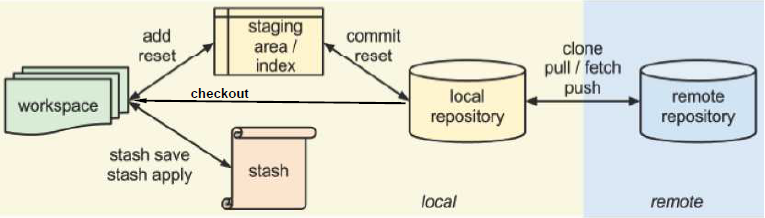
\includegraphics[width=11cm]{images/git.png}

\subsubsection{Git-Repository}
\begin{itemize}
	\item lokales Repository $\rightarrow$ \textit{".git"}-Verzeichniss im Workspace
	\item remote Repository $\rightarrow$ Git-Repository ohne Projektverzeichnis an externem Ort
	\item bare Repository $\rightarrow$ Git-Repository zum teilen, Klon von lokalen
\end{itemize}
\subsubsection{Git-Hashwerte}
\begin{itemize}
	\item Zur Identifizierung von Commits und Git-Objekten wird ein Hash-Wert generiert
	\item Hash-Wert wird mittels SHA1-Algorithmus generiert.
	\item die Hash-Werte werden als Zweigerwerte (Adressen) verwendet um die Repository-Datenstruktur aufzubauen
	\item Der Hashwert wird aus Dateiinhalt berechnet und für den Dateinamen verwendet
\end{itemize}
\clearpage
\pagebreak
\subsubsection{Git-Objekte}
	\begin{tabular}{|p{0.5\linewidth}|p{0.5\linewidth}|}
		\hline
		\begin{tabular}[c]{@{}l@{}}\textbf{blob}\\ -Inhalt einer Datei\\ -Keine Zeiger auf andere Objekte\end{tabular}   \newline  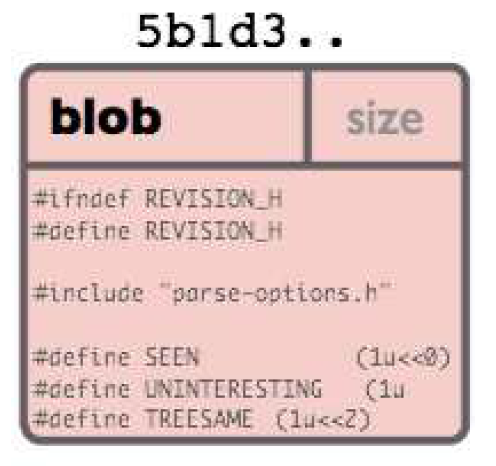
\includegraphics[width = 4cm]{images/blob}                             & \begin{tabular}[c]{@{}l@{}}\textbf{tree}\\ -enthält Zeiger auf blob-, oder tree-objekte\\ -enthält Information über Verzeichnis-,Dateinamen\end{tabular} \newline 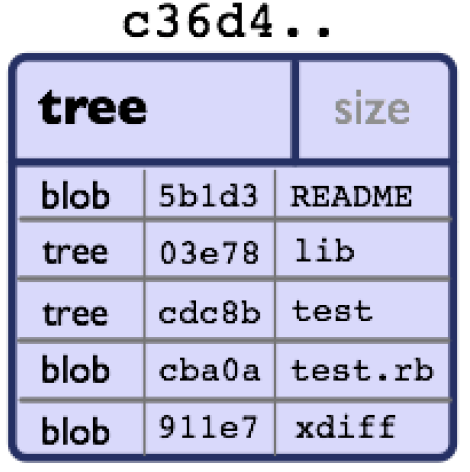
\includegraphics[width = 4cm]{images/tree} \\ \hline
		\begin{tabular}[c]{@{}l@{}}\textbf{commit}\\ -Startobjekt für ein Commit\\ -enthält Zeiger auf tree und vorgängiges commit-objekt\end{tabular} \newline 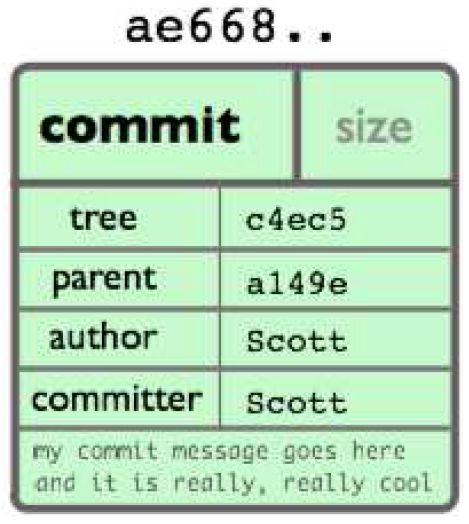
\includegraphics[width = 4cm]{images/commit}& \begin{tabular}[c]{@{}l@{}}\textbf{tag}\\ -Etikette mit Kommentar\\ -enthält Zeiger auf commit\end{tabular} \newline 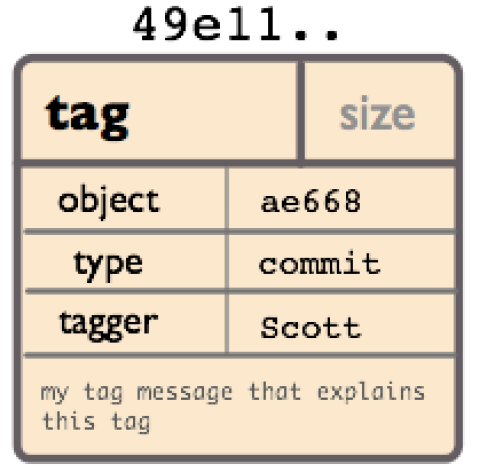
\includegraphics[width = 4cm]{images/tag}                                             \\ \hline
	\end{tabular}

\subsubsection{Git-Referenzen}
\begin{minipage}{12cm}
	\begin{itemize}
		\item Referenzen $=$ Zeiger (nur Zeigerwert)
		\item Zeigen nur auf Git-Objekte
		\item Hashwert-Zeiger $\rightarrow$ zeigt auf Branches/Tags
		\item Symbolischer-Zeiger $\rightarrow$ zeigt auf Datei mit Namen eines anderen Zeigers
	\end{itemize}
\end{minipage}
\begin{minipage}{6cm}
	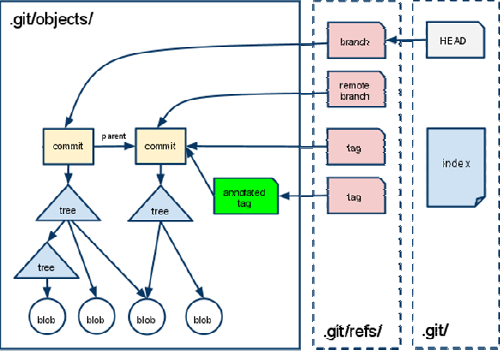
\includegraphics[width=6cm]{images/git-referenz.png}
\end{minipage}
\subsubsection{Bashprints}
\begin{multicols}{2}
	\begin{minipage}[l]{.40\textwidth}
		Files changed but not staged.\\    
		\textbf{\$ git status}\\
		On branch master\\
		Your branch is up-to-date with 'origin/master'.\\
		Changes not staged for commit:\\
		\quad (use "git add <file>..." to update what will be committed)\\
		\quad (use "git checkout -- <file>..." to discard changes in working directory)\\
		\\
		\qquad modified:\quad idiotenseite/IdiotenseiteInclude.tex\\
		\\
		no changes added to commit \newline (use "git add" and/or "git commit -a")\\
	\end{minipage}
	
	\begin{minipage}[r]{.40\textwidth}
		\textbf{\$ git log}\\
		commit 1b7ff854a491397087ff89689a535c275549e6ee\\
		Author: \quad Michel Gisler <Michel Gisler>\\
		Date:  \quad  Tue May 31 15:08:58 2016 +0200\\
		\\  
		\qquad Kleiner Ergänzungen und Anpasungen\\
	\end{minipage}
\end{multicols}
\clearpage
\pagebreak
\subsubsection{Git Commands}
\begin{longtable}{| p{.30\textwidth} | p{.70\textwidth} |}
	\hline 
	\textbf{Create}&
	\\ \hline
	
	git init <directory>&
	Create empty Git repo in specified directory.\newline
	Run with no arguments to initialize the current directory as a git repository.
	\\ \hline 
	
	git clone <repo>& 
	Clone repo located at <repo> onto local machine.\newline
	Original repo can be located on the local filesystem or on a remote machine
	\\ \hline  \hline
	
	\textbf{Local Changes}&
	\\ \hline 
	
	\hline 
	git status&
	List which files are staged, unstaged, and untracked  
	\\ \hline
	
	git diff& 
	Show unstaged changes between your index and working
	directory 
	\\ \hline 
	
	git diff HEAD&
	Show difference between working directory and last commit.
	\\ \hline
	
	git add <directory>&
	Stage all changes in <directory> for the next commit. Replace <directory>
	with a <file> to change a specific file or witch <.> to Stage all.
	\\ \hline 
	
	git commit -m " \" <message>"&
	Commit the staged snapshot, but instead of launching a text editor, use
	<message> as the commit message.
	\\ \hline
	
	git commit -a&
	Commit all local changes in tracked files.  
	\\ \hline 
	
	gitt commit --amend&
	Change the last commit. \textbf{Don‘t amend published commits!}
	\\ \hline \hline
	
	\textbf{Commit History}&  
	\\ \hline 
	
	\hline
	git log&
	Display the entire commit history using the default format.
	\\ \hline 
	
	git log -p <file>&
	Show changes over time for a specific file 
	\\ \hline
	
	git log --author="\"<pattern>"&
	Search for commits by a particular author. 
	\\ \hline
	
	git blame <file>& 
	Who changed what and when in <file>
	\\ \hline \hline
	
	\textbf{Branches and Tags}&  
	\\ \hline
	
	\hline
	git branch&
	List all of the branches in your repo. Add a <branch> argument to
	create a new branch with the name <branch>.
	\\ \hline 
	
	git branch <new-branch>&
	Create a new branch based
	on your current HEAD
	\\ \hline
	
	git branch -d <branch>&
	Delete a local branch
	\\ \hline   
	
	git branch -dr <remote/branch>&
	Delete a branch on the remote
	\\ \hline
	
	git checkout -b <branch>&
	Create and check out a new branch named <branch>. Drop the -b
	flag to checkout an existing branch.
	\\ \hline 
	
	git merge <branch>&
	Merge <branch> into the current branch.
	\\ \hline
	
	git tag <tag-name>&
	Mark the current commit with a tag (v1.0.1)
	\\ \hline  \hline
	
	\textbf{Update and Publish}&
	\\\hline 
	
	\hline
	git remote -v&
	List all currently configured remotes.
	\\ \hline 
	
	git remote add <name> <url>& 
	Add new remote repository, named <remote>
	\\ \hline 
	
	git fetch <remote>&  
	Download all changes from <remote>,
	but don‘t integrate into HEAD
	\\ \hline
	
	git pull <remote> <branch>&
	Download changes and directly merge/integrate into HEAD  
	\\ \hline 
	
	git push <remote> <branch>&
	Publish local changes on a remote
	\\ \hline \hline
	
	\textbf{ Merge and Rebase}&
	\\\hline 
	
	\hline
	git merge <branch>&
	Merge <branch> into your current HEAD
	\\ \hline 
	
	git rebase <branch>& 
	Rebase your current HEAD onto <branch>!\textbf{Don‘t rebase published commits!}
	\\ \hline 
	
	git rebase --abort&
	Abort a rebase
	\\ \hline 
	
	git mergetool& 
	Use your configured merge tool to solve conflicts
	\\ \hline \hline
	
	\textbf{Undo}&
	\\\hline 
	
	\hline
	git reset --hard HEAD&
	Discard all local changes in your working directory.
	\\ \hline  
	
	git checkout HEAD <file>&
	Discard local changes in a specific file
	\\ \hline   
	
	git revert <commit>&
	Revert a commit (by producing a new commit with contrary changes)
	\\ \hline    
	
	git reset <commit>&
	Move the current branch tip backward to <commit>, reset the staging area to match, but leave the working directory alone. 
	\\ \hline
\end{longtable}

\pagebreak
\section{Qt}
\begin{minipage}{16cm}
	Qt (sprich cute =süess) ist eine plattformübergreifende Programmierungsapplikation für grafische Benutzeroberflächen
    (GUI = Graphical User Interface).\\
	Qt wurde 1991 gegründet und gehörte der Firma Trolltech.
    Im Jahr 2008 übernahm Nokia die Firma Trolltech. Im Jahr 2014 wurde Qt als Open-Source-Projekt verwaltet. 
\end{minipage}
\begin{minipage}{1.5cm}
	
\includegraphics[width=1.5cm]{images/qt_logo.jpg}
\end{minipage}

\subsection{Grundlagen zu Qt}
\begin{minipage}{8cm}
	\begin{itemize}
		\item Qt C++ Klassenbibliothek stellt GUI-Elemente zur \newline Verfügung
		\item Das GUI wird als C++ Sourcefile geschrieben
		\item Standartklasse QtGui und QtCore werden automatisch inkludiert
		\item Alle Qt Widgets werden auf dem Heap erstellt
		\item Jedes Programm enthält eine Instanz von QApplication
		\item QApplication hält alles zusammen
		\item siehe Hello World Beispiel im Anhang für näheres
	\end{itemize}
\end{minipage}
\begin{minipage}{10cm}
	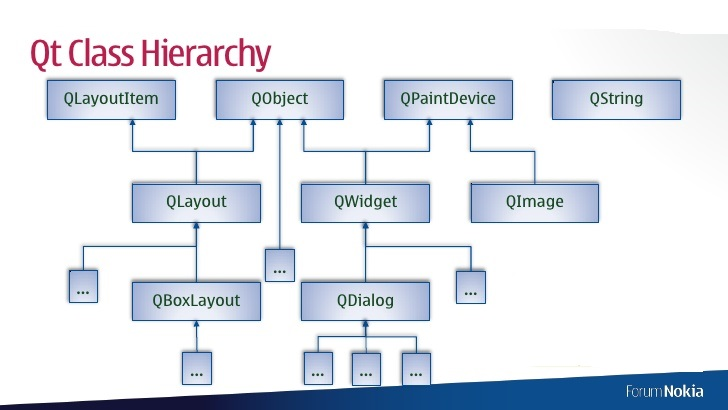
\includegraphics[width=10cm]{images/qt_classes.jpg}
\end{minipage}

\begin{multicols}{2}
	\subsubsection{QObject}
	\begin{itemize}
		\item QObject ist die Basisklasse des Qt-Modells
		\item stellt das Memorymanagement (automatische delete) für alle abgeleitet Klassen von QObject zur Verfügung. Es entstehen Objektbäume. 
		\item stellt die connect-Funktion zur Verfügung
		\item bearbeitet das Eventhandling
		\item hat keine visuelle Representation
	\end{itemize}
	
	\subsubsection{Qt Building}
	\begin{itemize}
		\item qmake Makefile-Generator
		\item macht aus plattformunabhängiem Projektfile (.pro) ein plattformspezifisches Projektfile. 
		\item die gewünschte Plattform wird qmake als Option mitgegeben
		\item Bei Build-Problemen alle Dateien\textbf{ausser} .pro und Sourcefile \newline löschen
	\end{itemize}
\end{multicols}

\subsubsection{Qt Konvention}
\begin{tabular}{|l|l|c|}
	\hline \textbf{Was}&\textbf{Beispiel} &\textbf{Konvention}
    \\ \hline   
    Qt-Modulname& "QtCore"&\textit{Qt}
    \\ \hline  
    Qt-Klassenname & "QString" &\textit{Q}
    \\ \hline   
    Qt-Variablen-,Funktionsname & "qTranslator, qDebug()"&\textit{q}
    \\ \hline   
    Qt-include & "\#include <QtGui>& \textit{ohne.h}
    \\ \hline
\end{tabular}

\subsection{QWidget}
\begin{itemize}
	\item abgeleitet von QObject,  eine Instanz der Klasse stellt grafisches Element dar
	\item Diese Klasse hat viele Methoden um Aussehen, Grösse, Position etc. zu verändern
	\item mit show() wird das Widget angezeigt, mit hide() wird das Widget versteckt
	\item Jedes Widget wird einem \textit{"Parent-Widget"} (Eltern) zugewiesen, ein solches Widgets nennt man dann \textit{Child-Widgets}
	\item Durch die Parent-Child Funktion entsteht eine Verschachtelung
	\item Ein Widget \textbf{ohne} Parent ist ein Top-Level-Widget oder Window	
	\item Das \textit{"Parent-Widget"} übernimmt Verwaltungsfunktionen wie Memory-Management, \newline
    weiterleiten von Ereignisse an \textit{"Child-Widget}, anzeigen, verstecken von Widgets etc.
\end{itemize}

\begin{multicols}{3}
\subsubsection{Top-Level-Widget}
Die \textit{"Top-Level-Window"} sind Widgets welche auf der obersten Hierarchiestufe liegen. Sie haben keine \textit{"Parent-Widget"}.\newline
Übliche Widgets für \textit{"Top-Level-Window"}: 
\begin{itemize}
	\item QMainWindow $\rightarrow$ Applikations-Window (Hauptfenster)
	\item QDialog $\rightarrow$ Popup-Window für Abfragen ("Wirklich löschen?"), Hauptanwendung bleibt blockiert
	\item QWidget $\rightarrow$ Einfaches Fenster
\end{itemize}

\subsubsection{Parent-Child-Widgets}
\begin{itemize}
	\item Jedes QObject kann maximal ein Eltern-QObject haben
	\item Jedes QObject kann beliebig viele \newline Kind-QObject haben
	\item Kind muss Eltern über sich informieren
	\item Entweder über Konstruktor, \newline label->setParent(mainwindow) oder Layout Manager
\end{itemize}

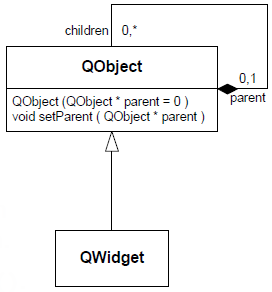
\includegraphics[width=5cm]{images/qt_parent_child.png}
\end{multicols}

\subsection{GUI-Programmierung}
Es gibt zwei grundlegende Aufgaben bei der GUI-Programmierung.\\
Das \textbf{Layout} legt Anordnung, Grösse  und Farbe fest.\\
Die \textbf{Interaktion} legt die Reaktion des Programmes auf eine Eingabe fest. \\

\subsection{Layout}
Es gibt drei Varianten wie Widgets innerhalb eines Widget angeordnet werden können: \newline
absolute Positionierung, Layout Manager und GUI-Designer (Qt Designer)

\subsubsection{Absolute Positionierung}
Mittels Methoden:
\begin{multicols}{2}	
	\lstinputlisting[style=c++qt]{source/Qt/methoden.cpp}
	
	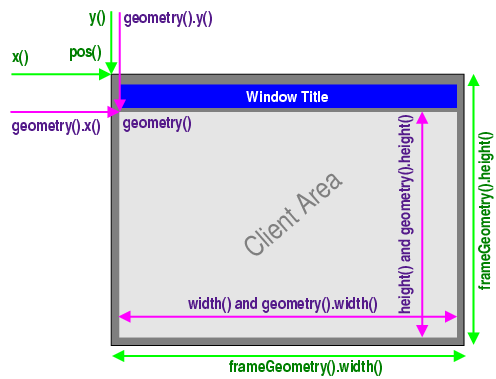
\includegraphics[width=7cm]{images/geometry.png}
\end{multicols}

\subsubsection{Layout Manager} %TODO Layout?
	\begin{tabular}{|l|l|}
		\hline \textbf{Klasse} & \textbf{Ort}\\
		\hline QVBoxLayout & Elemente vertikal\\
		\hline QHBoxLayout & Elemente horizontal\\
		\hline QGridLayout & zweidimensionales Gitter\\
		\hline QFormLayout & Elemente zeilenweise\\
		\hline QStackedLayout & aufeinandergelegt\\
		\hline
	\end{tabular}
	
\subsubsection{GUI-Designer / Qt Designer}	
	Anordnung innerhalb eines Formulars mittels interaktiven Tools, anschliessend Umwandlung in Code. 	

\subsection{Interaktion}
In Qt werden die Eingaben als SIGNALS bezeichnet und die Ausgaben als SLOTS. Mittels der Funktion connect() werden die beiden miteinander verknüpft.\\
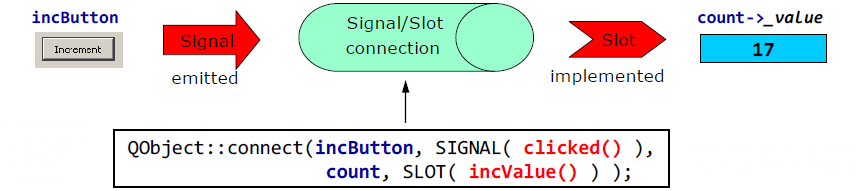
\includegraphics[width=15cm]{images/connect.png}

\begin{multicols}{3}
\subsubsection{SIGNALS}
\begin{itemize}
	\item nur deklariert, nie definiert
	\item kein Zugfriffsrecht vergeben
	\item Rückgabetyp immer void
\end{itemize}

\subsubsection{SLOTS}
\begin{itemize}
	\item deklariert und definiert
	\item oftmals Memberfunktion, auch normal abrufbar
	\item Zugriffsrechte
\end{itemize}

\subsubsection{connect}
\begin{itemize}
	\item Verbindungsfunktion zwischen Input und Output
	\item ein Signal zu mehreren Slots
	\item mehrere Signale zu einem Slot
\end{itemize}
\end{multicols}

\vspace{0.5pt}
\textbf{Beispiele connect-Funktion}
\lstinputlisting[style=c++qt]{source/Qt/connect.cpp}

\subsection{Zeichnen und Malen}
\begin{multicols}{2}
	\subsubsection{QPainter}
	Der Maler mit Mal-,\& Zeichenwerkzeugen.\\
	
	\begin{tabular}{|l|l|}
		\hline \textbf{Klasse} & \textbf{Werkzeug}\\
		\hline QPen & Zeichenstift\\
		\hline QBrush & Pinsel\\
		\hline QFont & Schriftart\\
		\hline draw & Formen malen\\
		\hline
	\end{tabular}
	
	\subsubsection{QPaintDevice}
	Oberfläche wo darauf gezeichnet \& gemalt werden kann
	QPainter-Objekte zeigen auf QPaintDevice-Objekte. QPaintDevice ist eine abstrakte Basisklasse welche nicht von QObject abgeleitet ist und daher \textbf{kein automatisches delete.}\\

\end{multicols}

\subsubsection{Vorgehen}
\lstinputlisting[style=c++qt]{source/Qt/qpainter.cpp}
\pagebreak
\section{Beispiele}

\subsection{CppUnit}
\lstinputlisting{source/CppUnit/AuthorTest.cpp}
\pagebreak

\subsection{Doxygen}
\textbf{Code} 
\lstinputlisting{source/Doxygen/Keyboard.h} 
\begin{tabular}{l l}
	\textbf{HTML-Dokumentation} & \textbf{Eclipse-Plugin}\\
	\tabbild[width=8cm]{images/doxygen_html.png} & \tabbild[width=10cm]{images/doxygen_basic.png}\\
\end{tabular}
\pagebreak

\subsection{Qt}
\subsubsection{Hello World}
\lstinputlisting{source/Qt/hello_world.cpp}
\subsubsection{QWidgets}
\begin{tabular}{c c}
	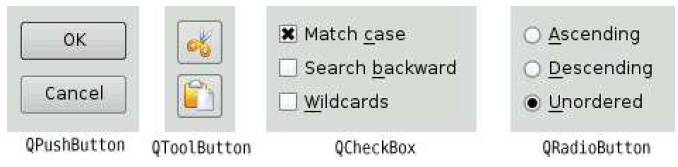
\includegraphics[width=9cm]{images/button_1.png}& 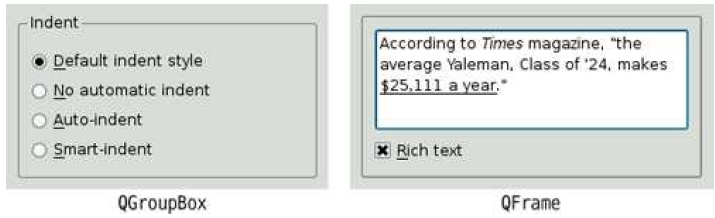
\includegraphics[width=9cm]{images/button_2.png}\\
	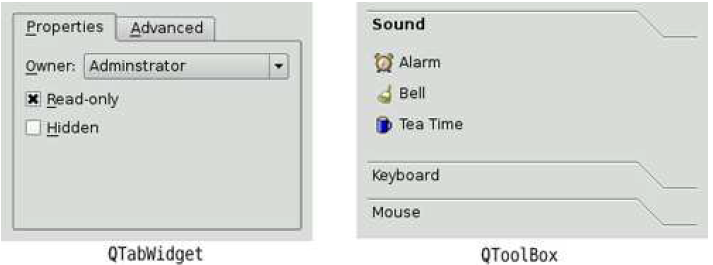
\includegraphics[width=9cm]{images/button_3.png}& 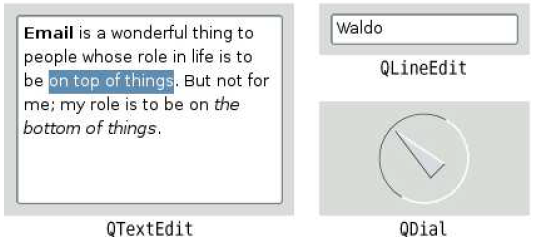
\includegraphics[width=9cm]{images/button_7.png}\\
	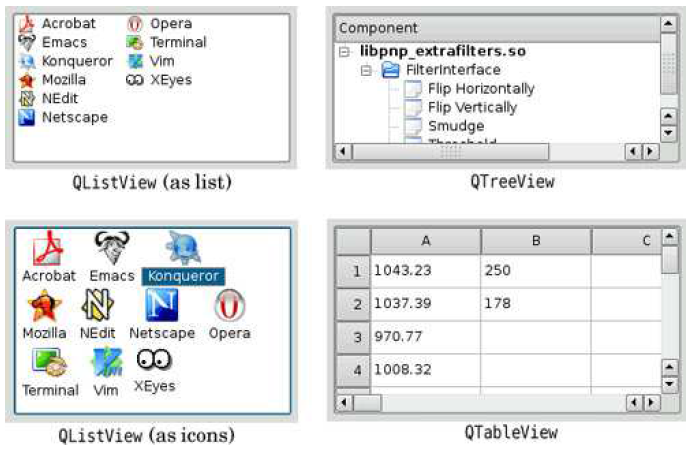
\includegraphics[width=9cm]{images/button_4.png}&
	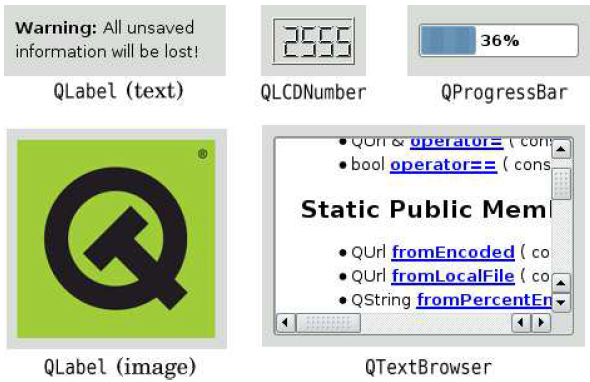
\includegraphics[width=9cm]{images/button_5.png}\\
	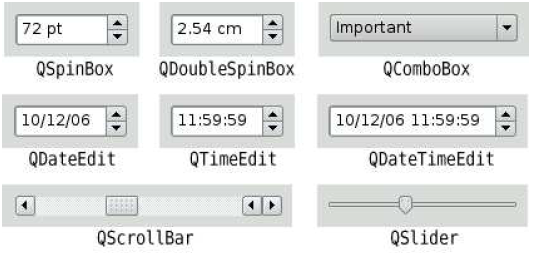
\includegraphics[width=9cm]{images/button_6.png}&
	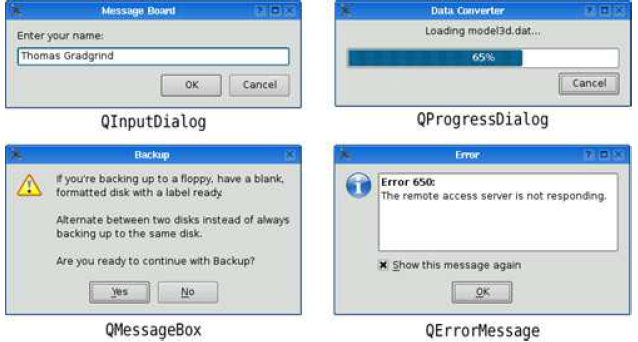
\includegraphics[width=9cm]{images/button_8.png}\\
\end{tabular}
\subsubsection{QBrush}
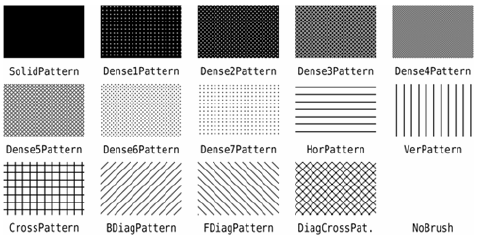
\includegraphics[width=9cm]{images/brush.png}

\subsubsection{QPainter draw-Methoden}
\begin{tabular}{c c}
	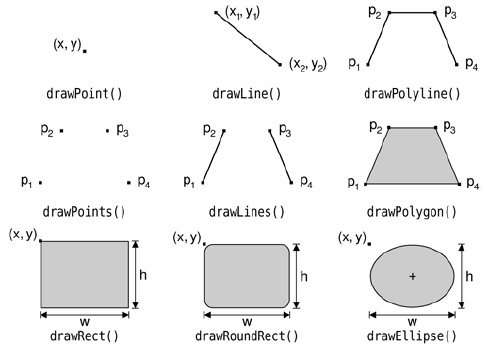
\includegraphics[width=9cm]{images/draw_1.png}& 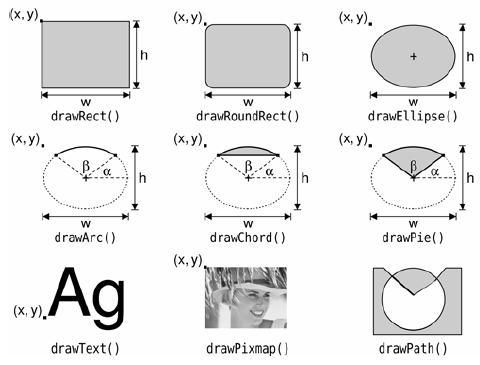
\includegraphics[width=9cm]{images/draw_2.png}\\
\end{tabular}
\subsubsection{QPen}
\begin{tabular}{c c}
	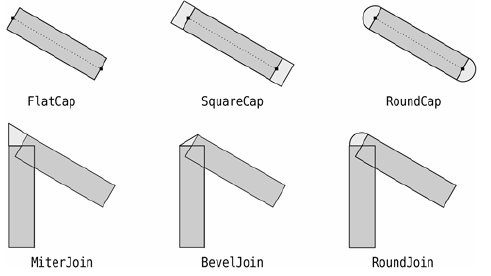
\includegraphics[width=9cm]{images/pen_1.png}& 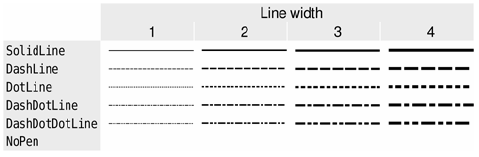
\includegraphics[width=9cm]{images/pen_2.png}\\
\end{tabular}
\newpage
\subsubsection{Temperaturwidget}
\textbf{main.cpp}
\\
\lstinputlisting{source/Qt/main.cpp}
\textbf{temperaturwidget.h}
\\
\lstinputlisting{source/Qt/temperaturwidget.h}
\newpage
\textbf{temperaturwidget.cpp}
\lstinputlisting{source/Qt/temperaturwidget.cpp}
\end{document}